\documentclass[brudnopis]{xmgr}

\usepackage{listings}
\usepackage{color}

\definecolor{dkgreen}{rgb}{0,0.6,0}
\definecolor{gray}{rgb}{0.5,0.5,0.5}
\definecolor{mauve}{rgb}{0.58,0,0.82}

\lstset{frame=tb,
  language=Java,
  aboveskip=3mm,
  belowskip=3mm,
  showstringspaces=false,
  columns=flexible,
  basicstyle={\small\ttfamily},
  numbers=none,
  numberstyle=\tiny\color{gray},
  keywordstyle=\color{blue},
  commentstyle=\color{dkgreen},
  stringstyle=\color{mauve},
  breaklines=true,
  breakatwhitespace=true
  tabsize=3
}

% tak można zmienić domyślną rodzinę fontów Latin Modern 
%   na Minion + Myriad + Monaco:
%\defaultfontfeatures{Scale=MatchLowercase}
%\setmainfont[Mapping=tex-text]{Minion Pro:+onum}
%\setsansfont[Mapping=tex-text]{Myriad Pro}
%\setmonofont[Scale=0.75]{Monaco}

\wersja   {wersja wstępna [\ymdtoday]}

\author   {Patryk Jażdżewski}
\nralbumu {186507}
\email    {pjazdzewski@inf.ug.edu.pl}

\title    {Testowanie hybrydowych aplikacji mobilnych}
\date     {2014}
\miejsce  {Gdańsk}

\opiekun  {dr W. Pawłowski}

\begin{document}

\begin{abstract}
  Poniższa praca zawiera opis biblioteki „Ash” służącej do funkcjonalnego testowania
hybrydowych aplikacji mobilnych stworzonych przy użyciu Adobe PhoneGap lub
Apache Cordova. Ash pozwala na testowanie zachowania się aplikacji w~różnorodnych
realistycznych scenariuszach, które bywają trudne do symulowania przez inne narzędzia, takich jak poruszanie się użytkownika,
obrót ekranu, utrata dostępu do sieci oraz~inne. Dzięki wykorzystaniu hybrydowego charakteru aplikacji
możliwa jest emulacja zachowania, co wpływa na większy realizm testów, a tym samym na wiarygodność ich wyników. Innymi
zaletami bliblioteki są elastyczna struktura testów, która ułatwia ich utrzymywanie oraz możliwość budowania złożonych scenariuszy z prostych kroków, a także
to, że pozwala na wykorzystania asercji w~aplikacji poza testami.
Możliwe jest także wykorzystanie Ash do testowania mobilnych wersji stron internetowych. 
\end{abstract}
\keywords{Javascript, 
 Apache Cordova, 
 Adobe Phonegap,
testowanie,
hybrydowe aplikacje mobilne}

% tytuł i spis treści
\maketitle

\introduction

Wstęp

\chapter{Wprowadzenie}
\section{Hybrydowe aplikacje mobilne}
Mówiąc o \textit{natywnej aplikacji mobilnej} mamy na myśli aplikację tworzoną z myślą o konkretnej platformie (Android, iOS, itp.) przy użyciu narzuconych przez twórcę platformy narzędzi (Java, Objective-C, itd.). Aplikacje mobile web są to z kolei aplikacje webowe zoptymalizowane po kątem urządzeń natywnych.
Adobe PhoneGap oraz jej odpowiednik o otwartym źródle Apache Cordova, to
dwie popularne biblioteki pozwalajace na tworzenie hybrydowych aplikacji
mobilnych, tj. aplikacji które łączą w sobie zalety aplikacji natywnych oraz \textit{aplikacji
typu mobile web}. Zasada działania tego typu aplikacji jest w założeniu prosta i
polega na wykorzystaniu komponentów, które dalej nazywać będziemy WebView.
Komponenty te są dostępne na każdej nowoczesnej platoformie i pozwalają na
wyświetalnie stron internetowych z wnętrza natywnych aplikacji mobilnych. 
W momencie startu aplikacja hybrydowa tworzy WebView oraz ładuje do niego zasoby z określonego adresu (lokalnego lub zdalnego), które są wyświetlane w WebView. Najczęściej tym zasobem jest aplikacja stworzona przy użyciu technologii webowych.     

% tabelki w LaTeX-u też da się robić, chociaż najczytelniej to może nie wygląda
% więcej na temt tabelek można poczytac np. na http://en.wikibooks.org/wiki/LaTeX/Tables
\begin{center}
    \begin{tabular}{ |  p{2cm} | p{4cm} | p{4cm} | p{4cm} |}
    \hline
   			& Aplikacje natywne        & Aplikacje hybrydowe 	& Aplikacje mobile web 			\\ \hline
    Narzędzia	& Zależne od platformy	&   Narzędzia webowe	& 	Narzędzia webowe			\\ \hline
    Instalacja	&        Wymagana               &	 Wymagana         	& 		Nie wymagana		\\ \hline
    Wydajność	& 	Bardzo dobra		&Ograniczona przez przeglądarkę&Ograniczona przez przeglądarkę\\ \hline
    Możliwość monetyzacji
    			&  Pobranie, reklamy, subskrybcje  & Pobranie, reklamy, subskrybcje & Reklamy, subskrybcje \\ \hline
    Dostęp do urządzenia
    			& 	Tak, pełen  	         &Najważniejsze funkcjonalności& Ograniczony        \\ \hline
    \end{tabular}
\end{center}

Takie podejście ma wiele zalet. Dzięki temu, że do tworzenia aplikacji hybrydowych wykorzystywane są technologie
znane z zastosowań intenetowych, koszt ich tworzenia i czas dostarczenia
gotowego rozwiązania na rynek są znacznie zredukowane. Aplikacje tego typu są też
z założenia wieloplatformowe. Używając PhoneGap z~tego samego kodu źródłowego
możemy stworzyć aplikacje na platformę Android, iOS, Blackberry, WebOS,
Windows Phone, Symbian i Bada. Dodatkowo popularność narzędzi internetowych
ułatwia znalezienie właściwych programistów.

\section{Wady podejścia hybrydowego}
Największymi wadami podejścia hybrydowego są słabsza wydajność, błędy
pojawiające się tylko na określonych urządzeniach oraz potencjalnie odmienne oczekiwania
użytkowników różnych platform. Użytkownik instalując aplikację hybrydową w taki sam sposób co 
natywną spodziewa się, że będzie ona działać niczym natywna. Tymczasem
dodatkowy narzut hybrydy, często w połączeniu z niechlujnie przygotowaną i nie
zoptymalizowaną aplikacją, prowadzi do mniej responsywnego interfejsu
użytkownika i w konskewencji do frustracji użytkownika. Częstym problemem przy
tworzeniu aplikacji mobilnych są błędy, które są specyficzne tylko dla pewnych modeli urządzeń. Przy podejściu hybrydowym problem jest o tyle bardziej widoczny, że
najczęściej tworzymy rozwiązanie które ma być przenośne nie tylko pomiędzy urządzeniami w ramach jednej platformy, ale także między platformami. Co z oczywistych względów zwiększa gamę urządzeń, które trzeba uzwględnić. Trzecim problemem hybryd jest kwestia
tworzenia interfejsu użytkownika. Dostawcy systemów operacyjnych dla urządzeń
mobilnych publikują zalecenia, co do tego jak powinien wyglądać interfejs aplikacji
działającej pod danym systemem. Zalecenia te są specyficzne dla platformy i często
wzajemnie się wykluczają. Przygotowanie jednej szaty graficznej i jednego interfejsu
może zostać źle odebrane przez użytkowników spodziewających się wyglądu
dostosowanego do platformy. Niestety stworzenie kilku wersji interfejsu jest dużo
bardziej pracochłonne i skomplikowane, niweczy także podstawową zaletę apliakcji
hybrydowych – przenośność. 
Są to poważne niedostatki, ale braki te można zniwelować z pomocą skutecznych narzędzi.

\section{Propozycja rozwiązania problemów}
Ash ma za zadanie pomóc rozwiązywać problemy zwiąne z wydajnością aplikacji oraz z
błędami zależnymi od konfiguracji sprzętowych. Aby
zapewnić wysoką sprawność działania aplikacji konieczny jest rygor przy tworzeniu
oprogramowania oraz możliwość testowania jej w sytuacjach, które pozwalają
uwydatnić problemy z wydajnością. Dzięki funkcyjnemu podejściu do testowania
oprogramowania Ash pozwala zbierać informacje o responsywności interfejsu
oraz realistycznie symulować scenariusze dużego obciążenia. Programista
korzystający z Ash ma możliwość zdefiniowania w scenariuszach maksymalnego
czasu przebeigu testu, jeśli test nie zakończy się w założonym czasie test nie
powiedzie się. Niska responsywność interfejsu traktowana jest na równi z błędami
logiki czy prezentacji. Wymusza to na twórcy zadbanie o szybkość reakcji interfejsu.
Ash oferuje także możliwość chwilowego wyłączenia lub opóźnienia dostępu do
sieci. Sytuacje w których dostępność internetu jest ograniczona są dość częste,
jednak niewiele aplikacji jest pisanych biorąc to pod uwagę, a jeszcze mniej 
testowana pod tym kątem. Bardzo często problemy z dotępem objawiają się kiepską
wydajnością interfejsu lub długimi przestojami na ekranach ładowania. Ash pozwala
twórcom świadomie zmierzyć się z tym problemem. Ash wyposażony jest w
mechanizmy pozwalajace na łatwe uruchomienie aplikacji na wielu urządzeniach
naraz, fizycznych jak i wirtualnych, także w zdalnych lokalizacjach. Sprawia to, że
użytkownicy są mają możliwość masowego uruchamiania testów na wszystkich
dostępnych im urządzeniach oraz są bardziej skłonni skorzystać z testów w czaseie
swojej pracy. Możliwość zdalnego uruchomienia testów daje możliwość stworzenia
rozproszonej bazy urządzeń, co pozwoli na testowanie także mniej typowych
konfiguracji.

\section{Dlaczego Apache Cordova}
Jako bazę do implementacji wybrałem Apache Cordova. Apache Cordova jest to
wersja PhoneGap, którą korporacja Adobe (właściel praw do PhoneGap) udostępniła
fundacji Apache. Od tego momentu ten wariant technologii udostępniany jest
zasadzie otwartego źródła. Pomimo tego oba projekty są niemal identyczne, a jedyna faktyczna różnica między nimi jest natury prawnej. Głównym powodem
wyboru tej technologii jest spory udziała w rynku hybrydowych aplikacji mobilnych,
dynamizm rozwoju oraz liczna społeczność.

\section{Test Driven Development}

Test Driven Development jest to metodologia wytwarzania oprogramowania opierająca się na krótkich cyklach programistycznych, o których często mówimy red-green-refactor:
\begin{itemize}
  \item RED Programista pisze testy automatyczne, pokrywające funkcjonalność, która została wyspecyfikowana, ale nie została jeszcze zaimplementowana. Na tym etapie testy nie przechodzą
  \item GREEN Następnie programista implementuje brakujące funkcjonalności, aż wszystkie testy napisane w poprzednim kroku stają się zielone, czyli uruchamiają się bez błędów
  \item REFACTOR Po zakończeniu implementacji tworzone są dodatkowe testy do istniejących już funkcjonalności. Sama funkcjonalność też jest udoskonalana
\end{itemize}

Dzięki zastosowaniu krótkich cykli oraz automatycznych testów metodologia ta pozwala na tworznie oprogramowania, które ma przemyślaną architekturę oraz spełnia wszystkie założenia. Testy automatyczne, które powstają podczas cyklu zwiększają prawdopodobieństwo, że w przypadku, gdy kod aplikacji zmieni się potencjalne błędy zostaną od razu wychwycone. 

Test Driven Developement jako metodologia jest powiązana z Extreme Programming oraz z koncepcją "Tests First", która zakłada że zestawy testów automatycznych powinny być tworzone jeszcze przed napisaniem tesotwanej aplikacji, co skutkuje wysoką jakością tworzonego oprogramowania.   

Test Driven Developement zostało spopularyzowane przez Kenta Becka.

Więcej informacji można znaleźć na:

\url{http://www.agiledata.org/essays/tdd.html}

\url{http://msdn.microsoft.com/en-us/library/aa730844(v=vs.80).aspx}

\section{Hierarchia testów}

Wyróżniamy wiele rodzajów testów:
\begin{itemize}
  \item Jednostkowe. Testy obejmujące poszczególne funkcje na najniższym poziomie. Ich wykonywanie musi być możliwie jak najszybsze. Nie powinny korzystać z zewnętrznych zasobów
  \item Integracyjne. Ten rodzaj testów pokrywa wiele komponentów aplikacji na raz i testuje nie tylko, czy każdy z poszczególnych działa poprawnie w izolacji, ale także czy komunikacja między nimi jest poprawna
  \item Funkcyjne. Testy tego typu sprawdzają, czy interfejs prezentowany użytkownikowi jest poprawny oraz czy interakcja z użytkownikiem działa poprawnie. U podstaw działanie tych testów leży symulowanie zachowania użytkownika
  \item A/B. Tak zwane testy A/B polegają na testowaniu oprogramowania pod kątem wygody i praktyczności interfejsu
  \item Wydajnościowe. Jak sama nazwa wskazuje służą one do sprawdzenia wydajności aplikacji
  \item oraz inne ...
\end{itemize}

W przypadku poprawnie zarządzanego projektu trzy pierwsze rodzaj tworzę hierarchię zwaną "piramidą testowania". Dwa pozostałe z wymienionych przeze mnie rodzajów pełni funkcję uzupełniającą. 

\begin{figure}[p]
    \centering
    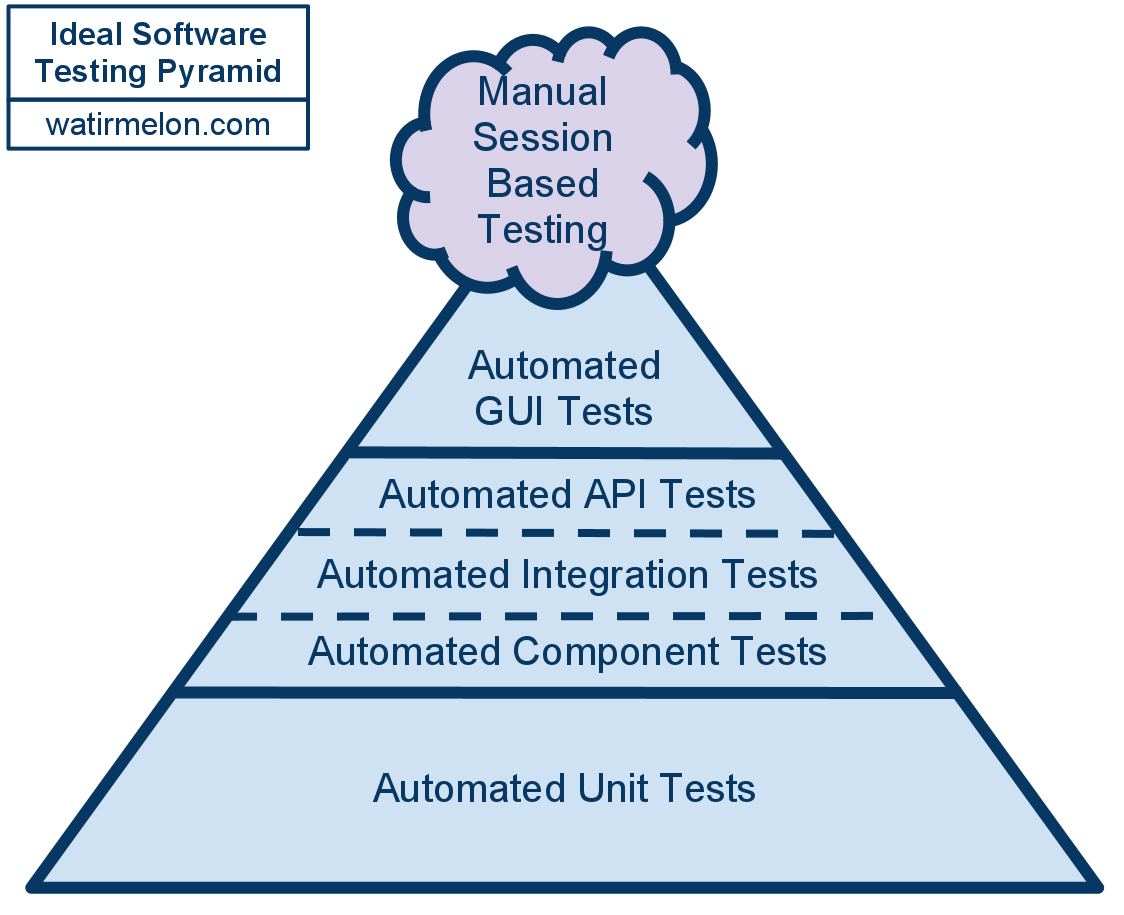
\includegraphics[scale=0.25]{idealautomatedtestingpyramid.png}
    \caption{Piramida testów}
    \label{fig:pyramis}
\end{figure}

Informacje na temat rozkładu piramidy testów oraz ich rozkładu w apliakcji można znaleźć tutaj:

\url{http://martinfowler.com/bliki/TestPyramid.html}

\url{http://www.duncannisbet.co.uk/test-automation-basics-levels-pyramids-quadrants}

Biblioteka Ash została stworzona z testowaniem funkcjonalnym na myśli.

\chapter{Sposób użycia}
\section{Getting Started}

Aby dołączyć Ash do swojego projektu wydaj następujace polecenie\footnote{Jeśli nie masz jeszcze zainstalowane Cordova CLI spójrz tutaj https://github.com/apache/cordova-cli}:
\begin{quote}
   cordova plugins add https://github.com/pjazdzewski1990/Ash
\end{quote}

Wtyczka zostanie zainstalowana, a do globalnej przestrzeni dodany zostanie obiekt Ash, który udostępnia wszystkie metody biblioteki.

Punktem startowym Ash jest metoda loadTests. Metoda ta przyjmuje tablicę ścieżek do plików zawierająych kod z testami i po wywołaniu dynamicznie dodaje wskazane pliki do dokumentu w ramach którego został wywołany. Pliki z testami należy napisać samodzielnie pamiętając, żeby były one zamknięte w ramach self-invocing-function. Celem takiego podejście służy do tego, żeby umożliwić użytkownikowi wpięcie i odpięcie testów z aplikacji oraz aby testy niepotrzebnie nie zaśmiecały aplikacji produkcyjnej.

Projekt demonstrujący użycie Ash oraz jego możliwości jest dostępny pod adresem

\url{https://github.com/pjazdzewski1990/AshDemo}

\section{Hello World}

Na porzeby wprowadzenia do testowania Ash powstała apliakcja AshHello, która jest dostępna pod adresem 

\url{https://github.com/pjazdzewski1990/AshHello}

Aby pobrać projekt 

\begin{quote}
   git clone git@github.com:pjazdzewski1990/AshHello.git
\end{quote}

Aplikacja AshHello zawiera w sobie bardzo prostą funkcjonalność. Jej zasadniczym celem jest pozwolenie użytkownikowi na zaznajomienie się z testowaniem przy użyciu biblioteki Ash. Interfejs użytkownika w AshHello jest zorganizowany na zasadzie tzw. {\it Working Square}. Working Square jest to wzorzec tworzenia interfejsu bardzo popularny na urządzeniach mobilnych. Polega on na stworzeniu kwadratowego obszaru roboczego który zawiera główną treść aplikacji oraz obszary pomocniczego na którym znadować się mogą np. elementy związane z nawigacją. Z zależności od orientacji ekranu, która dyktuje nam rozmiar i kształt powierzchni do zagospodarowania, obszar pomocniczy może znajdować się 

\begin{itemize}
  \item poniżej obszaru głównego - gdy urządzenia jest w orientacji pionowej, tzn. wysokość ekranu jest większa niż jego szerokość

\begin{figure}[p]
    \centering
    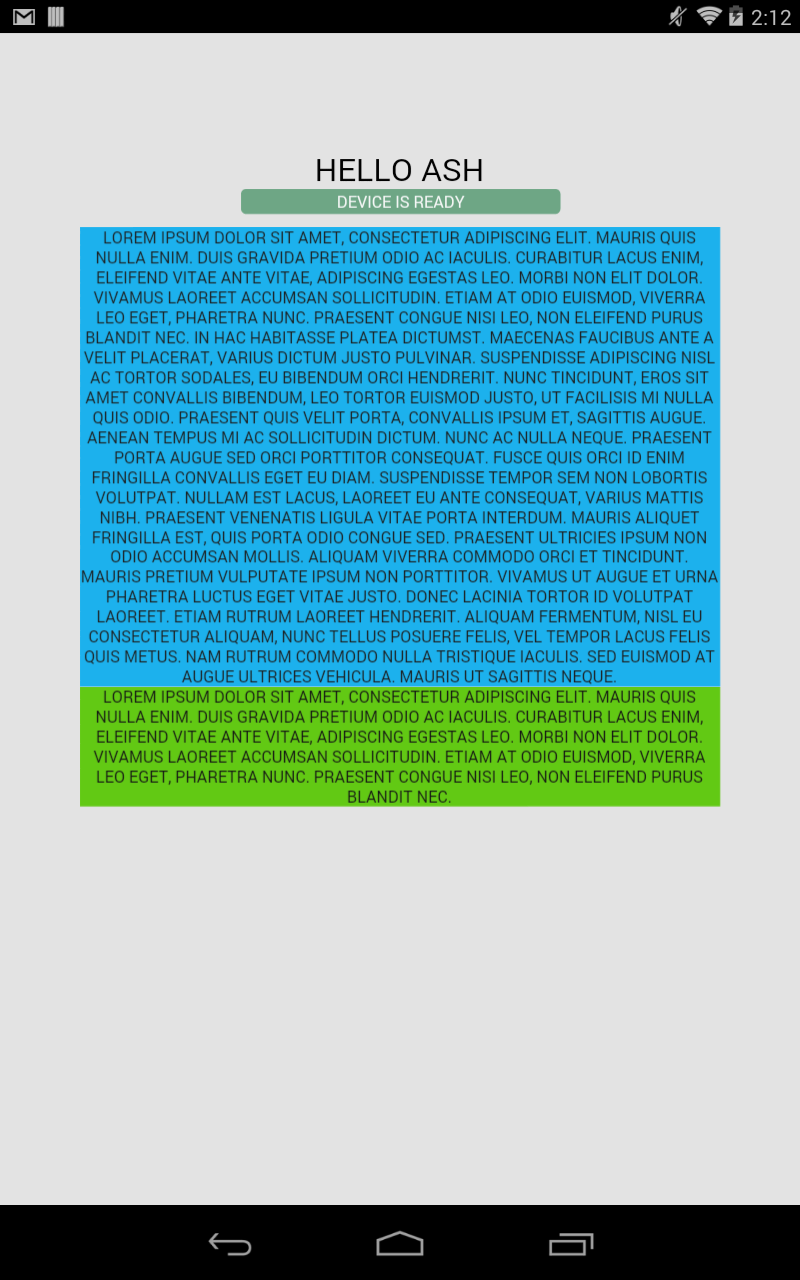
\includegraphics[scale=0.25]{hello1.png}
    \caption{AshHello w orientacji pionowej}
    \label{fig:AshHello1}
\end{figure}

  \item obok obszaru głównego - gdy urządzenie jest w orientacji poziomej, czyli szerokość dostępnego ekranu jest większa niż jego wysokość 

\begin{figure}[p]
    \centering
    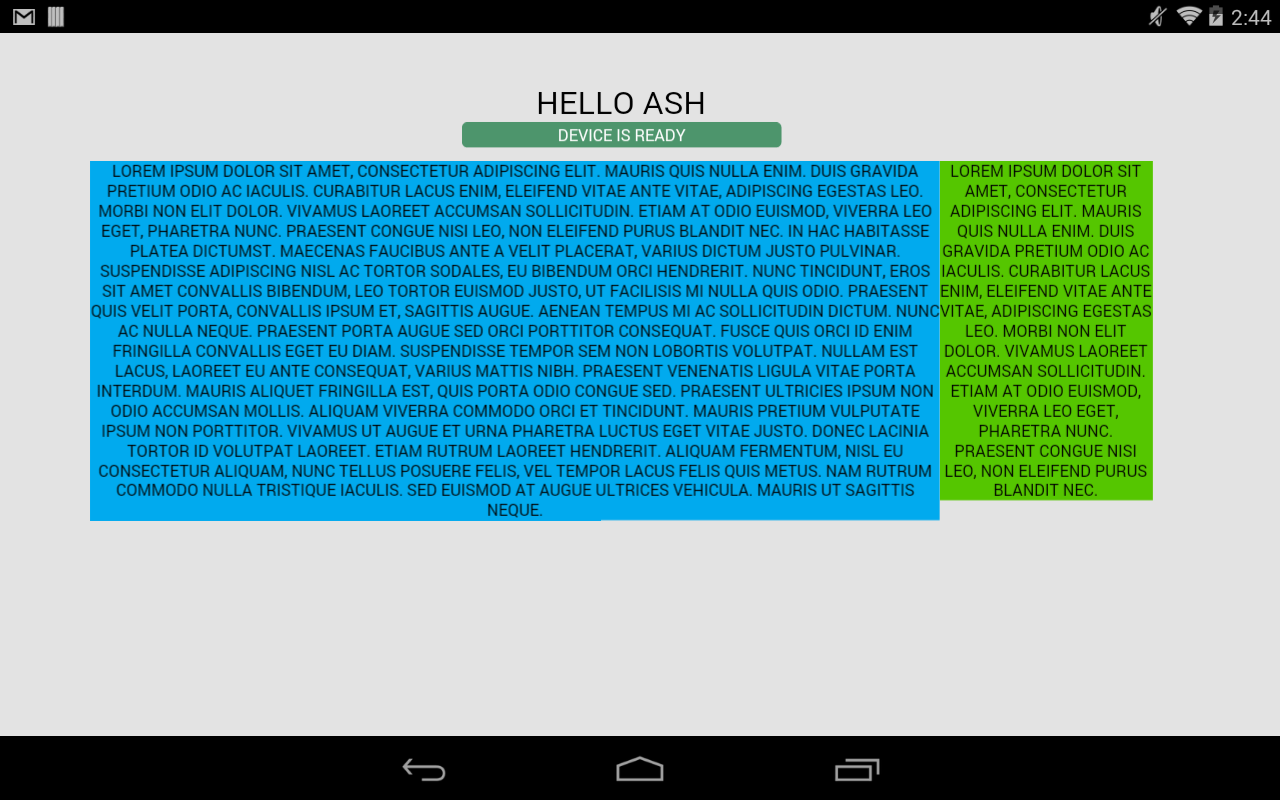
\includegraphics[scale=0.25]{hello2.png}
    \caption{AshHello w orientacji poziomej}
    \label{fig:AshHello2}
\end{figure}
\end{itemize}

Poniższa intrukcja krok po kroku wyjaśni, jak dodać testy Ash do projektu AshHello. Dla większej przejrzystości demonstracji testy będą korzystać z jquery, ale dołączenie tej biblioteki nie jest wymagane, gdy pracujemy z Ash.  

\begin{enumerate}
  \item Dodajemy Ash do projektu korzystając z Cordova CLI.\footnote{Projekt jest dostępny do pobrania pod adresem https://github.com/apache/cordova-cli}

Wtyczkę instalujemy poleceniem 
\begin{quote}
   cordova plugins add https://github.com/pjazdzewski1990/Ash
\end{quote}
i jeśli wszystko przebiegło poprawnie, to zmienna window.Ash powinna zawierać obiekt udostępniający funkcjonalność biblioteki.  

 \item Tworzymy plik z testami

W folderze www/ tworzymy katalog test/ a w nim plik myTest.js. W przed chwilą stworzonym pliku definiujemy samowywołującą się funkcję, która będzie zawierać nasze testy. Możemy to zrobić na przykład w ten sposób:

 \begin{lstlisting}
  (function(){
	console.log("MyTest started!");
	// tu znajdzie sie kod testujacy
  })();
\end{lstlisting}

Tak zdefiniowana funkcja zostanie wywołana zaraz po jej wczytaniu. Nasze testy nie będą bardzo skomplikowane, więc pozwolimy sobie na umieszczenia całej logiki bezpośrednio w tej funkcji. W przypadku bardziej rozbudowanych aplikacji i testów warto zgromadzić kodu obiekty.

Mamy zamiar sprawdzić, czy Working Square działa poprawnie w obu ustawieniach ekranu, więc musimy skorzystać z kontekstów 

\begin{quote}
   Ash.orientationHorizontal()
\end{quote}

oraz 

\begin{quote}
   Ash.orientationVertical()
\end{quote}

które pozwalają na odwrócenie ekranu. Możemy z nich skorzystać w następujący sposób

 \begin{lstlisting}
  //myTest.js

  Ash.orientationHorizontal().then(function(msg){
     //ten kod bedzie wywolany, gdy ekran znajdzie sie w orientacji poziomej
      var worksquare = $('.worksquare');
      Ash.assert(worksquare);
      
      var sidebar = $('.sidebar');
      Ash.assert(sidebar);

      Ash.equal(worksquare.getBoundingClientRect().top, sidebar.getBoundingClientRect().top);
     Ash.assert(worksquare.getBoundingClientRect().left < sidebar.getBoundingClientRect().left);

      Ash.endTest();
    });  
\end{lstlisting}

Powyższy test sprawdza trzy rzeczy. Po pierwsze znajduje elementy interfejsu, które chcemy zbadać. Przy użyciu Ash.assert() upewnia się, czy istnieją. A następnie porównuje ich pozycje upewniąjąc się, że lelementy są ułożone obok siebie i we właściwej kolejności. Ostanią operacją jest Ash.endTest() co oznacza zakończenie testu sukcesem.

Taki test obejmuje tylko część funkcjonalności. Musimy też zadbać o orientację pionową oraz o to, czy przejście nie ,,psuje'' interfejsu. Aby to zbadać możemy podpiąć dalszą część testu. Na przykład w ten sposób

 \begin{lstlisting}
  //myTest.js

  Ash.orientationHorizontal().then(function(msg){
       //kod z porzedniego punktu

      //to jeszcze nie koniec testu, wiec musimy zakomentowac lub usunac endTest()
      //Ash.endTest();
  }).then(
      Ash.orientationVertical //a teraz odwroc ekran pionowo
    ).then(function(msg){
      var worksquare = $('.worksquare');
      Ash.assert(worksquare);
      
      var sidebar = $('.sidebar');
      Ash.assert(sidebar);

      Ash.assert(worksquare.getBoundingClientRect().top < sidebar.getBoundingClientRect().top);
      Ash.equal(worksquare.getBoundingClientRect().left, sidebar.getBoundingClientRect().left);        

      //jesli aplikacja dotarla tutaj, to zaliczmy ten przypadek testowy
      Ash.endTest();
    });
\end{lstlisting}

Powyższy kod nie jest bardziej skomplikowany od poprzedniego. Jedyną nowością jest zastosowanie wielu bloków then(), które są wykonywane jeden po drugim w kolejności podania i pozwalają łączyć nam mniejsze funkcje testujace w bardziej złożone bloki.

 \item Dodajemy wywołanie kodu testującego do aplikacji

Teraz kiedy mamy już kod testów czas dodać go do aplikacji. W przypadku AshHello dobrym na to miejscem będzie index.js i metoda onDeviceReady(). Metoda ta jest wywołana, gdy zajdzie już zdarzenie 'deviceready' więc jesteśmy w stanie skorzystać z wszystkich dobrodziejstw Apache Cordova.

 \begin{lstlisting}
  //index.js
  
  var app = {
	...
    onDeviceReady: function() {
        console.log('Received onDeviceReady Event');
        app.setupUI();
        app.runAshTests();
    },
    runAshTests: function() {
        window.onerror = function(errorMsg, url, lineNumber) {
            alert("Error " + url + ":" + lineNumber + "\n" + errorMsg);
        };
        Ash.loadTests(["test/myTest.js"]);
    },
	...
  };

\end{lstlisting}

Nasza metoda runAshTests() robi dwie rzeczy dodaje wywołanie zwrotne dla zdarzenia onerror. W tym uproszczonym scenariuszu chcemy, żeby wszystkie błędy znalezione objawiały się wyskującym okienkiem z opisem problemu. Następnie korzystając z dotarczonej przez Ash metody loadTests() ładujemy myTests.js, jeśli przypomnimy sobie jak skonstruowany jest ten plik jasne stanie się, że od razu po wczytaniu zostanie on uruchomiony. 

\end{enumerate}

Tak niewiele potrzeba, żeby stworzyć i uruchomić pierwszy prosty test Ash. W razie problemów z uruchomieniem działający kod testowy znajduje się w branchu ,,with-tests''.

\section{Podejście do tworzenia testów}

Ash oferuje dużą swobodę jeśli chodzi o tworzenie zestawów testów przez użytkowników, jednocześnie sugeruje dobre techniki, które pozwalają w pełni wykorzystać możliwości biblioteki. W tym podrozdziale opiszemy kilka z tych zalecanych praktyk.    

\begin{itemize}
  \item Konteksty - wyzwalają określone zachowanie urządzenia, co pozwala nam na sprawdzenia jak zachowuja się nasza aplikacja np. w przypadku braku połączenia lub naciśnięcia przez użytkownika przycisku powrotu. Do konteksu możemy przekazać dowlną funkcję, która zostanie wywołana dopiero gdy urządzenie znajdzie się w określonym przez kontekst stanie. Konteksty stosujemy w ten sposób:

\begin{lstlisting}
  Ash.makeDeviceDoABC().then(function(msg){
      //sprawdz jak aplikacja sprawuje sie, gdy zaszlo zdarzenie ABC
      
      //zakoncz kontekst
      Ash.endTest();
  });
\end{lstlisting}

Powyższy kod działa dokładnie tak jak się go czyta. Ash wymusza na urządzeniu przejście w okreslony stan lub wykonanie pewnej czynności. Wtedy (,,then'') następuje wywołanie funkcji, która jest wywoływana już po przejściu i może ona sprawdzić zachowanie aplikacji. Bloki then można ze sobą łączyć. W takim wypadku kolejne bloki będą wykonywane jeden po drugim. Then może być także użyte do komponowania kontekstów. Jeśli przywołamy pewien kontekst X to do bloku them po nim następującego możemy przekazać funkcję wywołującą Y. W takiej sytuacji kolejne bloki then będą wykonywane, w sytuacji gdy X i Y będą zachodzić.  

Istotną rzeczą na którą należy zwrócić uwagę jest 

\begin{lstlisting}
   Ash.endTest();
\end{lstlisting}

Funkcja testująca może działać w sposób asynchroniczny lub być zagnieżdżona w innej funkcji. W takiej sytuacji trudne bywa ustalenie, kiedy zakończyła się przekazana funkcja. Funkcja endTest() pełni rolę informacyjną - wskazuje gdzie znajduje się punkt końcowy oraz pozwalają na zakończenie testu i uruchominie kolejnego z zestawu. Każdy test Ash powinien kończyć się wywołaniem tej funkcji. Jej brak może uniemożliwić wykonanie się serii testów, natomiast w przypadku uruchomienia tej funkcji poza testami po cichu zakończy ona działanie. O endTest() można myśleć jak o poleceniu do którego wykonania dążą testy i po którego wykonaniu test traktowany jest jako wykonany. 

Musimy też pamietać, że o ile stan urządzenia jest zdefiniowany w obrębie kontekstu, to poza nim już tak nie jest. Taka decyzja projektowa ma promować tworzenie testów, które są  niezależne od siebie i od warunków zewnętrznych wynikających z urządzenia.

  \item Page Objects - jest to wzorzec projektowy pozwalający na zapanowanie nad złożonymi interfejsami użtykownika i ich modularne testowanie. W Ash wykorzystywane są głównie do nawigacji po aplikacji. Pojedynczy Page Object reprezentuje element interfejsu np. stopkę, panel boczny, menu. Kilka takich obiektów składa się na ekran aplikacji. W Ash Page Object jest każdy obiekt, posiadający funkcje validate() oraz goto().

validate() zwraca wartość boolowską określającą, czy na obecnym ekranie znajduje się element interfejsu za który odpowiada dany Page Object. Z tej metody możemy skorzystać, aby upewnić się, czy całe bloki interfejsu są wyświetlone i czy są wyświetlone poprawnie.

goto() definiuje funkcje, która odpowiada za przejście przez aplikację, tak żeby rozważany Page Object stał się dostępny. Funckja powinna korzystać z validate(). goto() może być zastosowane np. do zmiany stanu interfejsu przed lub po teście.

Oczywiście Page Objects mogą zawierać także inne metody zdefiniowane przez użytkownika, które ułatwią operowanie na interfejsie z poziomu testów oraz uczynią kod testów czytelniejszym.

Prostota implementacji ma na celu uławienie korzystania z biblioteki, zachęca także do łączenia Page Objects ze sobą. Nic nie stoi na przeszkodzie, żeby zdefiniować Page Object ,,Menu'' jako zestaw kilku Page Objects, z których każdy opisuje jakiś element menu. 

 \item Organizacja testów - Zestawy możemy wykonywać albo przez polecenie run do którego przekazujemy tablicę funkcji-testów lub obiekt z testami (wtedy zgodnie z przyjętą konwencją uruchamianie są wszystkie funkcje, których nazwa kończy się frazą 'Test') albo korzystając z funkcji play wywoływanej ze scenariuszem testowym.

Scenariusz testowy, jest to w gruncie rzeczy tablica obiektów, które nazywamy krokami scenariusza. Na każdy krok składa się kilka informacji 

  \begin{itemize}
    \item name - możemy (ale nie jest to wymagane) podać nazwę kroku, ułatwi to czytanie informacji o błędach
    \item where - zawiera Page Object, do którego trzeba przejść, aby móc wykonać krok 
    \item what - tablica testów, które należy wykonać w tym kroku
    \item howLong - limit czasu na wykonanie testu, ustawienie odpowiednich limitów chroni nas i naszę apliakcję przed niezauważoną utratą wydajności
  \end{itemize}

Scenariusze pozwalają nam na tworzenie bardziej realistycznych przypadków użycia oraz wyrażanie ich w kodzie. 

\end{itemize}

\section{Ograniczenia}

Ash został stworzony w sposób na tyle elastyczny, aby był w stanie integrować się najróżniejszymi projektami. Niestety nie zawsze możliwe było uwzględnienie wszystkich możliwości, dlatego konieczne było przyjęcie pewnych założeń co do projektu który ma być testowany przez Ash. Zrozumienie tych założeń jest istotne do sprawnego posługiwania się biblioteką, zrozumienia przyczyn trudności w jej używaniu oraz przy podejmowania decyzji czy dołączyć Ash do swojego projektu.

Założnie Ash co do projektu testowanego:

\begin{itemize}
  \item wykonany w technologii Adobe Phonegap/Apache Cordova - istnieje możliwość aby w przyszłości testować także aplikacje typu mobile web, ale na obecnym etapie nie jest to celem Ash
  \item single page app - Ash zakłada, że aplikacja testowana będzie pisana zgodnie z najnowszymi trendami w branży oraz zaleceniami twórców Phonegap
  \item android 4.0+ - obecnie Ash pozwala testować jedynie aplikacje bazujące na Androidzie jako platformie, gdyż ta jest dominująca na rynku, ale w niedalekiej przyszłości planowana jest także wersja na iOS
\end{itemize}

\chapter{Przegląd funkcjonalności}

W każdej chwili istnieje możliwość wygenerowania aktualnej dokumentacji wprost z kodu aplikacji przy użyciu skryptu gen-doc.sh\footnote{Wymaga sh oraz zainstalowania programu jsdoc}

\section{Asercje}

\subsubsection{Sposób użycia}

Zestaw funkcji pomocniczych użytecznych podczas tworzenia testów.

\begin{quote}
Ash.assert( ... ) 
\end{quote}

\begin{quote}
Ash.assert( A, B ) 
\end{quote}

\begin{quote}
Ash.visible( ... ) 

Ash.isVisible( ... )

Ash.invisible( ... )

Ash.isInvisible( ... )
\end{quote}

\subsubsection{Opis}

Funckje assert są podstawowymi funkcjami z których tworzymy testy. Pozwalają one na 

\begin{itemize}
  \item sprawdzenie czy obiekt istnieje - funkcja assert(object) pozwala na sprawdzenie czy przekazany obiekt istnieje. Asercja ta zakłada, że każdy przekazany obiekt, który nie jest "falsy" z znaczeniu znanym z Javascript jest poprawny. 
  \item porównanie dwóch wartości - assert(A, B) sprawdza, czy oba podane arguemnty są identyczne wykorzystując do tego porównanie dokładne, tzn. bierzemy po uwagę typ, wartość oraz nie wykonujemy konwersji obiektów celem porównania.
\end{itemize}
Powyższe asercje w przypadku, gdy argumenty nie spełniają założeń rzucają ustandardyzowane wyjątki Ash. 

Funkcja widzialności visible(A) określają czy przekazany element DOM jest widoczny na ekranie, tzn. czy jego właściwości nie wskazują na to, że jest ukryty oraz czy nie jest poza widocznym ekranem. Analogicznie obiekt spełnia invisible(A), gdy nie spełnia visible(A). 

Różnica pomiędzy funkcjami X oraz isX jest taka, że te pierwsze rzucają wyjatki Ash, gdy założenie nie jest spełnione, natomiast te drugie tylko zwracają wartość boolowksą określającą czy arguemnt spełnia założenia.  

\section{Zmiana położenia ekranu}

\subsubsection{Sposób użycia}
Pozwala ustawić ekran w określonym położeniu - landscape/horizontal lub portrait/vertical.

\begin{quote}
Ash.orientationHorizontal().then( ... ) 
\end{quote}

\begin{quote}
Ash.orientationVertical().then( ... ) 
\end{quote}

\subsubsection{Opis}

Smartfony i tablety ze względu na swój mobilny charakter oraz dotykowy ekran bardzo często używane są w pozycjach i w sposób, o których twórcom nawet się nie śniło. Najczęściej rozróżniamy dwie pozycje definiujące położnie ekranu wzgledem użytkownika. 

\begin{itemize}
  \item pionowe - gdy  TODO
  \item poziome - gdy TODO
\end{itemize}

Każda dobrze wykonana aplikacja powinna uwzględniać te dwie pozycje. W każdej z nich przestrzeń, którą mamy do dyspozycji jest w prawdzie taka sama, ale jej posterzganie przez użytkownika jest inne, dlatego należy inaczej rozmieścić elementy interfejsu.  

Funkcje orientationHorizontal oraz orientationVertical  ustawiają ekran na pozycjach, odpowiednio, poziomej oraz pionowej względem domyślnej pozycji "zero" urządzenia. Pozycja ta może, ale nie musi być tą pozycją w której w momencie wołania znajduje się ekran.  

Należy pamiętać, że poza kontekstem orientationX status ekranu nie jest określony. Może być on dowolny. W szczególności wykonanie testu z orientation nie musi po fakcie nie musi przywracać poprzedniego ustawienia. Celem takiego podejścia jest wymuszenie na użytkowniku biblioteki zamykanie całego kodu związanego z położeniem w kontekście obrotu ekranu. 

Praktycznym podejściem może być sprawdzanie jak na zmianę ekranu reagują pojedyncze części ekranu zamiast całość. innym podejściem jest przetestowanie jak aplikacja reaguje na zmianę położenia ekranu a następnie na jego powrót. Można to zrealizować w ten sposób:

\begin{lstlisting}
   //example.js

  Ash.orientationHorizontal().then(function(msg){
      //sprawdz czy interfejs jest ulozony dla pozycji poziomej
    }).then(
      Ash.orientationVertical
    ).then(function(msg){
      //sprawdz czy interfejs jest ulozony dla pozycji pionowej
      Ash.endTest();
    });
  };
\end{lstlisting}

\section{Dostęp do sieci}

\subsubsection{Sposób użycia}

Daje możliwość manipulowania dostępem do sieci - pozwala blokować dostęp do sieci.

\begin{quote}
Ash.noNetwork().then( ... ) 
\end{quote}

\begin{quote}
Ash.slowNetwork().then( ... ) 
\end{quote}

\begin{quote}
Ash.networkOn().then( ... ) 
\end{quote}

\subsubsection{Opis}

Większość aplikacji mobilnych korzysta w ten czy inny sposób z zasobów zgromadzonych na zdalnych serwerach. W wielu przypadkach komunikacja z serwerem jest najistotniejszym  czynnikiem wpływającym na szybkość oraz poprawność działania aplikacji. Niestety za względu na mobilny charakter urządzeń dostęp do sieci bardzo często bywa utrudniony lub wręcz niemożliwy, co gorsza dzieje się tak nie regularnych ostępach czasu w zależności od czynników zewnętrznych. Dlatego kluczowe znaczenie ma przetestowanie w jaki sposób zachowa się aplikacja, gdy z jakiegoś powodu nie możliwe będzie nazwiązanie połączenia. Właśnie taką możliwość udostępnia Ash. 

\begin{lstlisting}
   //example.js

   Ash.noNetwork().then(function(msg){
      ...
      Ash.equal($('#connectionField').text(), 'No network connection');
      Ash.endTest();
    });
  };
\end{lstlisting}

W kontekście noNetwork dostęp do sieci zostanie zablokowany i nie możliwe będzie skomunikowanie się z zewnętrznymi serwisami.

Testując brak dostępu do internetu warto zwrócić uwagę nie tylko na to co dzieje się w przypadku, gdy żądanie nie powiedzie się ale także jak szybko się to stanie. Może dojść do sytuacji, gdy aplikacja testowana, w przypadku braku internetu, będzie wysyłać zapytania do serwera i czekać na upływ limitu czasu lub powtarzać je do skutku. W takiej sytuacji płynność działania aplikacji może ulec znacznemu pogorszeniu lub w najgorszym przypadku aplikacja może zmusić użytkownika do czekania na odpowiedź serwera, która nigdy nie nadejdzie. Jeśli chcemy zabezpieczyć się przed utratą płynności w przypadku ograniczenia dostępu do internetu istnieje możliwość skorzystania z pola 'howLong' w specyfikacji scenariusza testowego, tzn. możemy skonfigurować testy w ten sposób, że jeśli czas ich trafania przekroczy wybraną przez nas wartość test się nie powiedzie. Za wspomnianą wartość możemy przyjąć taką ilość czasu, po której użytkownik może poczuć dyskomfort. 

Podobną funkcjonlaność jak noNetwork() oferuje kontekst slowNetwork(). Jedyną różnicą jest to, że w przypadku tego kontekstu sieć jest dostępna, z tym że wszystkie żadania są opóźnione, tak jak w przypadku słabych połączeń. Sztucznie dodane kilku sekundowe spowolnienie sprawia, że jesteśmy w stanie symulować utrudnienia przy korzystaniu z sieci, które nie powodują całkowitej utraty połączenia. 

Należy zwrócić uwagę że, w zależności od implementacji, po wyjściu z kontekstów noNetwork() oraz slowNetwork() dostęp do sieci nie musi być przywrócony. Celem przywrócenia urządzenia do poprzedniego stanu należy skorzystać z kontekstu networkOn(). 

Kontekst networkOn() służy do przywrócenia domyślnego stanu sieci. W żadnym wypadku nie powoduje podłączenia do sieci, a jedynie powrót do stanu sieci sprzed manipulacji przez Ash. W obrębie tego kontekstu możemy być pewni, że dostęp do internetu nie jest utrudniony bardziej niż to wynika z czynników zewnętrznych. 

W przypadku gdy do testowanej aplikacji dodane jest wtyczka cordova-plugin-network-information,  to po wywołaniu kontekstu slowNetwork() oraz networkOn() zachodzi zdarzenie 'online'. Analogicznie w przypadku kontekstu noNetwork() wysyłane jest zdarzenie 'offline'. 

\section{Dostęp do systemu plików}

\subsubsection{Sposób użycia}
Pozwala realizować scenariusze testowe zakładające operowanie na plikach.

\begin{quote}
var options = { type: 'audio/amr', limit: 3};

Ash.withFile(options).then( ... )
\end{quote}

\subsubsection{Opis}

Bardzo częstym scenariuszem w przypadku wielu aplikacji jest konieczność operowania na lokalnym systemie plików. Może to być np. upload pliku z karty SD, wykonanie zdjęcia i przesłanie na serwer lub inne. Ash daje możliwość przetestowania jak aplikacja zachowuje się przy operowaniu na plikach.  

Do kontekstu withFile przekazujemy obiekt zawierający informacje na jakich plikach chcemy przeprowadzić testy. Obiekt może posiadać następujące klucze:

\begin{itemize}
  \item type - Jest to ciąg znaków, który określa jakiego typu mają być zwrócone pliki. Domyślnie jest to 'audio/amr' czyli plik dźwiękowy. 
  \item limit - Limit jest to wielkość plików w zwracanej tablicy wyrażony liczbą całkowitą. W przypadku, gdy limit nie został podany tablica zawiera 1 element. 
\end{itemize}

WithFile zwraca obiekt Promise. W przypadku realizacji obietnicy do bloku przekazywana jest tablica plików która może być wykorzystana w testach. Każdy plik w jest identyczny i spełnia założenia podane w argumencie 'options'. Przykładowy plik z tablicy może wyglądać w ten sposób:

\begin{lstlisting}
   {
       "name": "file1",
       "fullPath": "/path/to/file1",
       "type": "audio/amr",
       "lastModifiedDate": "Thu Apr 24 2014 22:52:29 GMT+0200 (CEST)",
       "size": 100
   };
\end{lstlisting}

Co odpowiada definicji pliku w ujęciu Apache Cordova. Patrz:

\url{https://cordova.apache.org/docs/en/3.0.0/cordova_file_file.md.html#File}

\section{Symulacja ruchu}

\subsubsection{Opis}
Ash dostarcza API umożliwiające symulowanie położenia lub ruchu między dwoma punktami.

\subsubsection{Sposób użycia}

\section{Obsługa przycisku powrotu}

\subsubsection{Sposób użycia}
Ta funkcjonalność symuluje naciśnięcie przycisku powrotu na telefonie. 

\begin{quote}
Ash.pressBack().then( ... ) 
\end{quote}

\subsubsection{Opis}

Integralną cześcią sytemu Android jest przycisk powrotu do poprzedniego ekranu. Specyfikacja systemu określa dokładnie

\begin{quote}
{TODO: umieścić wycinek speca tutaj}
\end{quote}

Niezależnie od dostawcy sprzętu, implementacji czy wersji systemu zastosowanie przycisku zawsze jest takie samo - pozwolić użytkownikom na łatwą nawigację w aplikacji, która będzie spójna pomiędzy najróżniejszymi aplikacjami. Bardziej precyzyjnie nawigacja w tym kontekście  oznacza możliwość powrot do poprzedniej aktywności lub ekranu prezentowanego użytkownikowi. W przypadku aplikacji hybrydowych opartych na Javascript oraz technologiach webowych powrót do poprzedniej aktywności oznacza cofnięcie stanu WebView do poprzedniego adresu URL. Wszystkie adresy dowiedzane przechowywane są na stosie, a ich unikalnośc determinowana jest przez 3 cześci adresu: hosta, ścieżkę oraz tzw. hash. 

\begin{lstlisting}
   //example.js

  var pressBackTest = function(){
    var pageOne = 1;
    var pageTwo = 2;
    // function app.mySwipe.slide(A, x) nawiguje do podstrony A w ciagu x milisekund,
    // po zakonczonej nawigacji hash adresu jest zmieniany
    app.mySwipe.slide(pageOne, 1); 
    app.mySwipe.slide(pageTwo, 1); 
    app.mySwipe.slide(pageTwo + 1, 1); // wykonujemy 3 ruchy, zeby moc cofnac sie 2 razy i wrocic do punktu wyjscia
    
    Ash.pressBack().then(function(msg){
      Ash.equal("#" + pageTwo, window.location.hash);
    }).then(
      Ash.pressBack
    ).then(function(){
      Ash.equal("#" + pageOne, window.location.hash);
      Ash.endTest();
    });
  };
\end{lstlisting}

Ash pozwala na cofanie się aż do szczytu stosu historii aplikacji. W szczególności od razu po uruchomieniu aplikacji nie możliwe jest wykonie pressBack. W takiej sytuacji pressBack nie powiedzie się, ale nie dojdzie także do wyjścia z aplikacji.

Testowanie obsługi przycisku powrotu na olbrzymie znaczenie w przypadku apliakcji mobilnych  oraz tzw. "Single Page Applications". Tworząc aplikacje bardzo wiele uwagi jest poświęcane sytuacjom kiedy użytkownik porusza się niejako "w głąb" aplikacji otwiera kolejne ekrany na zaplanowanej ścieżce zmieniając jej stan.  Właśnie globalny stan bywa w takich sytuacjach problemem. Bardzo często bywa, że użytkownik przechodzi przez ekrany A i B, w czasie swojego pobytu na B zmienia globalny stan, ale zamiast przechodzić dalej cofa się do A, które od czasu zmiany stanu zachowuje się inaczej niż zakładano. Tworząc aplikację należy zabezpieczyć się przed takimi sytuacjami. Ash.pressBack pozwala na przetestowanie czy taka sytuacja ma miejsce. 

\chapter{Zastosowania}
Ash został pomyślany jako biblioteka, która jest w stanie oprócz dostarczania ,,tradycyjnej'' infrastruktury testowej, tzn.:
\begin{itemize}
  \item asercji
  \item funkcji porównujących
  \item loggerów
  \item narzędzi do budowania testów
  \item ustandaryzowanych wyjątków
\end{itemize}
ułatwić także tesotwanie sytuacji, które są albo trudne do odtworzenia
\begin{itemize}
  \item operacje na plikach
  \item badanie widoczności elementu na ekranie
\end{itemize}
 albo w poza możliwościami typowych rozwiązań testujących
\begin{itemize}
  \item ustawienie ekranu urządzenia
  \item dostęp do sieci
  \item symulowanie ruchu
\end{itemize}
Ash może z powodzeniem być stosowany zarówno jako osobny (standalone) i samodzielny framework testujący, jak i uzupełnienie innych rozwiązań. W ogólnym ujęciu Ash jest przeznaczony do fukcyjnego testowania aplikacji, tzn. aplikacja jest testowana od strony interfejsu użytkownika, co ma swoje zalety (najbardziej wiarygodnie symuluje użytkownika) jak i wady (interfejs często podlega zmianom). Jak zostało wcześniej wspomniane testy funkcyjne dają najlepsze efekty, gdy są uzupełniane przez testy jednostkowe.  

\section{Problemy związane z obecnymi rozwiązaniami}

Obecnie istniejące rozwiązania pozwalajace na funkcyjne testowanie hybrydowych aplikacji mobilnych nie są wystarczające. Większość z nich wywodzi się z technologii webowych co ogranicza ich zastosowanie tylko do tej części aplikacji, która odpowiada aplikacji typu mobile web. Rozwiązania te nie są w stanie wykorzystać przewagi jaką daje hybrydowe podejście Apache Cordova, nie są w stanie ani przetestować ani skorzystać z natywnych podwalin aplikacji hybrydowej. W naturalny sposób ogranicza to ich możliwości oraz zastosowanie w kontekście rozważanych aplikacji. Naturalną wadą wielu bibliotek do funkcyjnego testowania aplikacji jest ich wrażliwość na zmiany interfejsu użytkownika. W przypadku większości aplikacji warstwa interfejsu jest tą częścią, która zmienia się najczęściej. W konsekwencji pożądaną własnością dobrej biblioteki do testowania funkcyjnego jest abstrakcja pozwalajaca na oderwanie się od detali interfejsu użytkownika oraz prostota pozwalająca na łatwą zmianę testów, gdyby zaszła taka potrzeba. 
                                                                                                                                                                                                                                                                                                                                                                                                                                                                                                                                                                                                                                                                                                                                                                                                                                                                                                                                                                                                                                                                                                                                                                                                                                                                                                                                                                                                                                                                                                                                                                                                                                                                                                                                                                                                                                                                                                                                                                                                                                                                                                                                                                                                                                                                                                                                                                                                                                                                                                                                                                                                                                                                                                                                                                                                                                                                                                                                                                                                                                                                                                                                                                                                                                                                                                                                                                                                                                                                                                                                                                                                                                         
\section{Ash jako rozwiązanie}

Ash jest biblioteką służącą do funkcyjnego testowania hybrydowych aplikacji mobilnych, która stara się minimalizować niedostatki tego podejścia poprzez pełne wykorzystanie możliwości dawanych przez hybrydowy charakter testowanych aplikacji. 

Ash działa na zasadzie wtyczki do Apache Cordova jest więc w stanie komunikować się z platformą sprzętową poprzez Native Bridge. Daje to możliwość manipulowanie ustawieniami czy zasobami urządzenia np. uzyskania dostępu do systemu plików czy ustawień połączenia. System operacyjny na którym uruchomiona jest aplikacja hybrydowa ma spory wpływ na to jak zachowa się aplikacja, niestety tradycyjne podejścia nie pozwalają na przetestowanie ich wpływu na aplikację. Co innego Ash, który udostępnia funkcjonalności pozwalające na wywoływanie określonych zachowań urządzenia. 

Zewnętrzne API Ash napisane jest w jezyku Javascript i także w tym języku pisane są testy. Jestem zdania, że Javascript ze względu na swój charakter pozwoli w prosty i przejrzysty sposób wyrazić testy oraz będą one na tyle elastyczne, że wymagane zmiany będą mogły być wprowadzane niewielkimi nakładami sił. API Ash kładzie nacisk na na powtórne wykorzystywanie kodu oraz korzystanie ze wzorca Page Object, co pozwala na zapanowanie nad potrzebą aktualizacji testów do szybko zmieniającej się aplikacji. 

\section{RWE - real world example}

\chapter{Wtyczki}

Apache Cordova udostępnia swoje API na zasadzie wtyczek. Każda wtyczka może być indywidualnie instalowana oraz udostępnia określone API i związane z nim funkcjonalności. Takie podejście pozwala na rozbicie monolitycznego API na mniejsze części oraz zapewnia możliwość rozszerzenia platformy poprzez własne wtyczki.

Każda wtyczka składa się z dwóch części - API programisty napisanego w języku Javascript i udostępionego użytkownikom oraz warstwy kodu natywnego, który realizuje zadania niewykonywalne z poziomu WebView. Część natywna implementowana jest w technologiach zależnych od platformy. Przenośna wtyczka posiada kilka implementacji, w różnych językach, które sa podmieniane w czasie budowania aplikacji. Kod natywny jest opcjonalny dla wtyczek, ale korzystając z platformy istnieje możliwość wzbogacenia aplikacji.

Ash, został zaimplementowany jako wtyczka do platformy. Obecnie warstwa natywna jest przygotowana tylko dla platformy Android, ale dalszym etapie rozwóju biblioteki planowane jest dodanie wsparcia dla innych platform. Kod działający po stronie systemu Android został napisany w języku Java.

Więcej informacji można znaleźć w oficjalnej instrukcji dla twórców wtyczek

\url{http://cordova.apache.org/docs/en/edge/guide\_hybrid\_plugins\_index.md.html\#Plugin\%20Development\%20Guide}  

\url{http://cordova.apache.org/docs/en/edge/guide\_platforms\_android\_plugin.md.html\#Android\%20Plugins}   

Nastepne podrozdziały koncentrują się na implementacji na platformę Android, ale w przypadku innych systemów zasada działania jest zbliżona.

\section{Klasa CordovaPlugin}

CordovaPlugin jest to klasa, która jest rozszerzana przez każdą wtyczkę. Udostępnia ona dostęp do najważniejszych składowych aplikacji oraz komunikację z warstwą Javascript: 

\begin{itemize}
  \item CordovaWebView webView - komponent WebView w którym uruchomiona jest aplikacja
  \item CordovaInterface cordova - daje dostęp do zasobów platofrmy np. Activity oraz puli wątków
\end{itemize}

{TODO prosty diagram klas dla commitu b872df0f314194ad50cbaa098ebbf717e53bb354}

Punktem wejściowym dla kodu każdej wtyczki jest jest metoda exec, która jest wywoływana, gdy warstwa javascript wyśle żadanie wywołania określonego kodu natywnego. Sygnatura exec wygląda tak:

\begin{lstlisting}
public boolean execute(String action, JSONArray args, final CallbackContext callbackContext) throws JSONException
\end{lstlisting}

Kolejne argumenty to
\begin{itemize}
  \item action - nawza metody, która ma zostać wywołana
  \item args - argumenty wysłane z warstwy Javascript zakodowane w postaci JSON
  \item callbackContext - specjalna klasa Apache Cordova pozwalająca na wywoływanie zdarzeń po stronie WebView 
\end{itemize}

W kodu Javascript kod natywny możemy wywołać w następujący sposób:

\begin{lstlisting}
//Ash.js
var cordova = require('cordova');

cordova.exec( 
        successCallback,
        failureCallback, 
        "Ash", 
        "networkSlow", 
        []
);
\end{lstlisting}

Kolejne argumenty to
\begin{itemize}
  \item successCallback - wywołanie zwrotne uruchamiane, gdy odwołanie do natywnej części wtyczki się powiedzie
  \item failureCallback - wywołanie zwrotne uruchamiane, gdy odwołanie do natywnej części wtyczki zakończy się błędem
  \item pluginName - nazwa pluginu, będąca jego unikalnym identyfikatorem w obrębie aplikacji
  \item actionName - nazwa akcji, która ma być wywołana. Ten argument jest później przekazywany do exec() jako parametr name 
\item arguments - tablica argumentów wywołania przekazywana do exec() jako zmienna args 
\end{itemize}

\section{Wielowątkowość. Komunikacja między warstwami}

Javascript ze swojej natury jest jednowątkowy. Tak samo wszystkie testy w Ash są wykonywane jeden po drugim. Poza trudnościami technicznymi powodem takiego podejścia jest to, że wiele gdyby wątków rywalizowało o współdzielony zasób, jakim jest DOM, konieczne byłoby zadbanie o ich synchronizację, co jest skomplikowane oraz mało wydajne. Z prawdziwą wielowątkowością mamy do czynienia dopiero na poziomie natywnej platformy.

Wtyczki działają asynchronicznie. Kod uruchamiany po stronie natywnej platformy przez wywołania cordova.exec() działa w osobnym wątku. Realizuje on swoje cele a następnie poprzez CallbackContext uruchamia odpowiednie wywołania zwrotne przekazane przez użytkownika wtyczki. Takie podejście pozwala maksymalnie wykorzystać wiele wątków działających po stronie platformy bez komplikowania budowy aplikacji po stronie warstwy  JavaScript. W takim przypadku kod natywny nie wpływa bezpośrednio na WebView czy sposób interfejs apliakcji użytkownikowi. Wszelkie tego typu mainpulacje odbywają się po stronie Javascript za pośrednictwem funkcji zwrotnych. Niestety czasami istnieje konieczność bezpośredniej manipulacji WebView w taki wypadku istnieje możliwość skorzystania z metody runOnUiThread(). Metoda ta przyjmuje klasę implementującą interfejs Runnable, w której mozemy nadpisać metodę run() tak, aby realizowała nasze cele. Na przykład w ten sposób:

\begin{lstlisting}
//AshPlugin.java
cordova.getActivity().runOnUiThread(new Runnable() {
      public void run() {
           // .... tu mozna bezpiecznie operowac na WebView oraz interfejsie
      }
});
\end{lstlisting}

Komunikacja pomiędzy warstwami wtyczki, natywną oraz Javascript odbywa się przez tak zwaną "Native To Js Queue". Jak sama nazwa wskazuje komunikacja pomiędzy warstwami odbywa się za pomocą kolejki. Oba poziomy aplikacji mogą umieszczać zakodowane wiadomości w kolejce, ale tylko jedna wiadomość może być przetwarzana. Pozwala to uniknąć kłopotów z wielowątkowością. Konsekwencją takiej implementacji protokołu komunikacji jest to, że kluczowe znaczenie przy wywoływaniu kodu, który odwołuje się między warstwami ma kolejność w jakiej wiadomości zostaną umieszczone w kolejce. W szczególności kolejka nie jest priorytetowa i nie ma w niej pojęcia ,,ważności'' wiadomości, czyli nie możliwe jest przepuszczenie wiadomości przed innymi.

\chapter{Architektura}

Ash dystrybuowany jest jako wtyczka do Apache Cordova z tego korzysta on także ze wszystkich mechanizmów typowych dla tego typu rozwiązań. Po dołączniu wtyczki do projektu np. za pomocą Cordova Command Line Interface w projekcie dostępny staje się globalny obiekt Ash, udostępniający wszystkie funkcjonalności biblioteki. 

Pola globalnego obiektu można podzielić na 3 grupy:  
\begin{itemize}
  \item proste funkcjonalności działające w sposób synchroniczny
  \item fukcje działające asynchronicznie i udostępniające złożoną funkcjonalność 
  \item prywatne, wewnętrzne pola oraz funkcje biblioteki
\end{itemize}
Warto podkreślić, że trzecia grupa nie wchodzi w skład oficjalnego, publicznego API Ash. Oznacza to, że o ile wiele z tych funkcjonalności czy helperów może być przydatna dla twórców testów, to nie rozsądnym jest korzystanie z nich bezposrednio, gdyż w przyszłych wersjach aplikacji w zależności od potrzeb kod ten może zostać zmieniony w sposób, który zmieni jego zachowanie lub/oraz API, co spowoduje niekompatybilność kodu testów z nową wersją Ash.

\section{Spojrzenie z lotu ptaka}

Ash definiuje funkcje pozwalajace na uruchamianie testów w kontekście pewnego zdarzenia sprzętowego, tj. możemy przygotować test, co do którego będziemy pewni, że w czasie jego działania będą zachodzić określone okoliczności. Możemy na przykład stworzyć test, który zostanie wykonany w sytuacji braku sieci np. w ten sposób:

\begin{lstlisting}
     //example.js

   //zdefiniuj kontekst braku sieci oraz uruchom w jego ramach przekazana funkcje
    Ash.noNetwork().then(function(){
	// tu mozemy umiescic kod testu
     	// zostanie on wykonany z kontekscie braku dostepu do sieci

	//tu powinien znalezc sie kod testujacy zachowanie aplikacji 
    });
\end{lstlisting}

Blok then pozwala zdefiniować co nastąpi po tym, jak sieć zostanie wyłączona. Jest to bardzo ważny aspekt biblioteki. Mamy pewność, że przez cały czas działania funkcji zachodzić będzie określony warunek. Warto zwrócić uwagę na przykładzie, że o ile w ramach kontektu stan sieci jest precyzyjnie zdefiniowany, to poza tymi ramami już tak nie musi być, stan możmy traktować jako dynamiczny lub nieokreślony. Dodatkowo należy pamiętać, że zmiana ustawień urządzenia w ramach kontekstu nie musi pociągać za sobą jego zmiany po wykonaniu testów. Ma to duże znaczenie z perspektywy testowania aplikacji, gdyż niejako wymusza, żeby w ramach jednego konteksu testować jedynie te rzeczy, które są z nim związane, a elementy interfesju które od nie zależą poza tym kontekstem.

Warto zaznaczyć, że konteksty można ze sobą łączyć, aby tworzyć bardziej złożone scenariusze. Takie złączenie realizujemy poprzez wilelokrotne użycie funkcji 'then' wraz z funkcjami, które chcemy wywyłać. Pozwala to na zdefiniowanie na przykład takiego kontekstu:

\begin{lstlisting}
     //example.js

    Ash.noNetwork().then(
	Ash.orientationHorizontal
    ).then(function(arg){
      	// w tym momencie mozemy byc pewni, ze zachodza dwa warunki:
	// 1) dostep do sieci zostal odciety 
	// 2) ekran znajduje sie w pozycji horyzontalnej

	//tu powinien znalezc sie kod testujacy zachowanie aplikacji 
    });
\end{lstlisting}

możemy także wywołania funckcji Ash przeplatać innym kodem JavaScript np. w ten sposób:

\begin{lstlisting}
     //example.js

    Ash.orientationHorizontal().then(function(msg){
	// tu mozemy umiescic kod JavaScript
      	
	// ekran jest w pozycji horyzontalnej
      
	// tu mozemy umieccic kod JavaScript
      	Ash.orientationVertical().then(function(){
		// tu mozemy umiescic kod JavaScript

        		// ekran jest w pozycji wertykalnej 

		// tu mozemy umiescic kod JavaScript
      	});
    });
\end{lstlisting}

\section{Promises}

Wewnętrznie Ash korzysta z mechanizmu obietnic tzw. Promise. Promises jest to mechanizm pozwalający programistom w lepszy prostszy i bardziej przejrzysty sposób panować nad  asynchronicznością. Dotychasowe podejście do kodu wykonującego się w sposób asynchroniczny wymagało oprócz parametrów wywołania przekazania także dwóch wywołań zwrotnych. Jednego wołanego w przypadku sukcesu oraz drugiego w przypadku wystąpienia błędu. Promise działają inaczej wywołanie promise zwraca obiekt o którym możemy myśleć jak o obietnicy, że kiedyś będzie on zawierał wynik jakiejś funkcji. Z jednej strony ułatwia to myślenie o asynchronicznych wywołaniach, z drugiej pozwala nam na traktowanie przyszłych zdarzeń jak obiektów. To znaczy, że możemy przypiąć do nich jedną lub wiele funkcji, które będą wołane dopiero gdy wewnętrzne obliczenia zostaną zakończone. Możliwe jest też łatwe szeregowanie obetnic, co w przypadku tradycyjnego podejścia prowadziło do tzw. "callback hell", czyli zagłębiania funkcji w funkcjach do tego stopnia że stają się one absolutnie nieczytelne. 

Dokładny opis mechanizmu, jego wymagania oraz zastosowania można znaleźć na  stronie projektu

\url{http://promises-aplus.github.io/promises-spec/}

Na chwilę obecną nawet w samym JavaScript istnieje wiele implementacji specyfikacji Promises. W Ash pierwotnie zastosowano bibliotekę o nazwie promises.js dostępną pod adresem

\url{https://github.com/then/promise/}

Za tym wyborem przemawiał niewielki rozmiar kodu (co ogranicza narzut związany z dodawaniem dodatkowej biblioteki do projektu korzystajacego z Ash) oraz bogactwo funkcjonalności (promises.js wiernie implementuje specyfikację oraz wzbogacając ją o kilka  nowych możliwości). Niestety szybko okazało się, że funkcjonalności oferowane przez promises.js nie do końca odpowiadają wymaganiom projektu. Biblioteka nie została jednak porzucona, ale zamiast tego zaadaptowana do specyficznych potrzeb Ash.  

\section{Wzorzec Object Pages w Ash}

W celu nadania testom struktury oraz zwiększenia elastyczności testów biblioteka Ash korzysta ze wzorca projektowego Object Pages znanego na przykład z biblioteki Selenium. 

\url{https://code.google.com/p/selenium/wiki/PageObjects}

lub

\url{http://docs.seleniumhq.org/docs/06\_test\_design\_considerations.jsp\#page-object-design-pattern}

Page Object reprezentuje stan interfejsu użytkownika, pojedynczego komponentu lub zbioru komponentów. W praktyce Ash jako Page Object traktuje każdy obiekt, który definiuje dwie bezparametrowe funkcje zwracające wartości logiczne:

\begin{itemize}
  \item validate
  \item goto
\end{itemize}

Metoda validate wywoływana jest w celu sprawdzenia, czy obecny UI spełnia wymagania danego Page Object. Innymi słowy, czy metoda ta pozwala nam ustalić, czy znajdujemy się na właściwej podstronie. 

Metoda goto pozwala na przejście na ekran definowany przez dany obiekt. Metoda ta może wewnątrz korzystać z validate w celu upewnienia się czy już nie znajdujemy się na właściwej stronie. 

Oczywiście Page Objects można w sobie zagłębiać, na przykład jeden Page Object może zależeć od kilku mniejszych i jego metoda validate zakłada, że metody validate podstron będą spełnione. 

Prosty Page Object w Ash może wyglądać w ten sposób:

\begin{lstlisting}
     //example.js
    var somePageObject = {
    	validate: function(){
      	    var screen = document.getElementById('elementId');
             return Ash.isVisible(screen);
          },
         goto: function(){
             if(!this.validate()) app.mySwipe.slide(0, 1);
             return true;
         }
    };
\end{lstlisting}

\section{Organizacja testów. Run oraz Play}

Ash oferuje dwa podejścia do uruchamiania testów 'Run', o którym dalej będziemy nazywać "uruchamianiem testów" oraz 'Play', co dla rozróżnienia nazywiemy "odgrywaniem scenariuszy".

Obie wspomniane metody korzystają z wywołań zwrotnych raczej niż z podejścia wykorzystującego obietnice. Taka decyzja podyktowana jest tym, że 'Play' i 'Run' są  metodami najwyższego poziomu i nie ma powodu, żeby je łączyć ze sobą. Dodatkowo mechanizm promise w żaden sposób nie wymusza podania funkcji do obsługi zdarzeń, natomiast w tym przypadku chcemy mieć pewność, że zostały one podane.  

\subsubsection{Run}

Ten tryb oferuje proste API do szybkiego uruchamiania niezależnych od siebie testów. Sygnatura funkcji: 

\begin{quote}
function Ash.run(array[function] testsArray, function failureCallback[, function successCallback]) 
\end{quote}

Przykładowe zastosowanie: 

\begin{lstlisting}
     //example.js

    var exampleTests = [
	// tu umiesc funkcje z kodem testow
    ];

    Ash.run(exampleTests, function(errorData){
      // ten callback zostanie uruchomiony, za kazdym razem gdy test sie nie powiedzie
    }, function(successData){
      // ten callback jest opcjonalny, jesli zostanie podany to Ash uruchomi go za kazdym razem, gdy test sie powiedzie
    });
\end{lstlisting}

Run pozwala na sekwencyjne uruchomienie przekazanych testów w kolejności zgodnej z indeksem tablicy. Ash nie czyni żadnych zabiegów, aby testy nie kolidowały i nie ingerowały w działanie innych testów, dlatego testy przekazywane winny być od siebie nawzajem niezależne. Dostarczane one są do Ash jako tablica bezparametrowych funkcji.

Ash definiuje zestaw funkcji wyzwalaczy wołanych podczas uruchomienia Run. Funkcje te znajdują się w globalnym obiekcie Ash.callbacks, ale mogą być swobodnie nadpisywane przez użytkowników. Ich wywołanie następuje w ściśle zdefiowanych momentach, dzięki czemu użytkownik Ash może lepiej kontrolować przebieg testów. Typowy przebieg wywołania Ash.run wygląda w ten sposób:

\begin{itemize}
  \item Ash.callbacks.beforeClass
  \item Ash.callbacks.before
  \item {test dostarczony przez użytkownika}
  \item Ash.callbacks.after
  \item ....
  \item Ash.callbacks.before
  \item Test dostarczony przez użytkownika jest wywoływany
  \item Ash.callbacks.after
  \item Ash.callbacks.afterClass
\end{itemize}

Każdy z dostarczonych testów kończy się wywołaniem jednego z dostarczonych funckcji - obowiązkowego failureCallback wywoływanego jeśli z jakiegoś powodu test się nie powiedzie oraz opcjonalnego successCallback wołanego w momencie poprawnego wykonania się testu.

Do wywołań zwrotnych przekazywane są obiekty zawierające informacje o wykonaniu testu. Do errorCallback:

\begin{lstlisting}
	{
		"level": // string, wskazuje jak powazny jest problem, moze byc uzyty jako tag np. do filtrowania 
		"code": // int, kod bledu
		"message": // string, komunikat bledu 
		"url": // string, zawiera informacje w ktorym pliku doszlo do bledu 
		"lineNumber": // int, zawiera informacje gdzie w pliku doszlo do bledu
	}
\end{lstlisting}

Do successCallback: 

\begin{lstlisting}
	{
		"length": // int, ile testow znajduje sie na tablicy przekazanej do run 
		"index": // int, index obecnego testu w tablicy 
	}
\end{lstlisting}

\subsubsection{Play} 

Play jest wyższą formą uruchamiania testów niż run, ale tylko w sensie, że bazuje na run. Najważniejszą z różnic pomiędzy run a play jest to, że play wykonuje uporządkowany i zsynchronizowany zestaw testów, w którym to zestawie istnieje ściśle określona kolejność oraz zależność pomiędzy kolejnymi testami-krokami. Play pozwala na uruchomienie przygotowanego wcześniej scenariusza. 

Sygnatura funkcji play jest podobna do run:

\begin{quote}
function Ash.play(array[function] scenarioArray, function failureCallback[, function successCallback]) 
\end{quote}

Scenariusze przekazujemy jako tablicę obiektów na przykład:

\begin{lstlisting}
[
      {
          name: "First Step",
          where: somePageObject,
          what: [somePageTest],
          howLong: 1500	// in miliseconds
      },
      {
          name: "Second Step",
          where: otherPageObject,
          what: [otherPageTest],
          howLong: 1000	//in miliseconds
      }
  ];
\end{lstlisting}

każdy z obiektów musi defioniować następujące klucze:

\begin{itemize}
  \item PageObject where - określa na jakim ekranie aplikacji ma zostać uruchomiony test
  \item Array[Function] what - zestaw bezparametrowych funkcji, które będą wywoływane jedna po drugiej 
  \item Integer howLong - jak długo ma trwać wykonanie testów, jeśli przekroczony zostanie wyznaczony tu limit test zostaje uznany za niepowodzenie 
\end{itemize}

dodatkowo może definiować:

\begin{itemize} 
  \item String name - nazwa kroku scenariusza, ma zastosowanie pomocnicze
\end{itemize}

Kroki scenariusza przekazane do play wykonywane są przy użyciu wcześniej opisanej metody run, jeden po drugim w kolejności od mniejszych indeksów. Po każdym pojedynczym wykonaniu porównywane są czasy realny oraz założony przekazany jako klucz 'howLong'. W przypadku, gdy czas realny jest większy niż założony test oznazany jest jako niepowodzenie. Biblioteka Ash definiuje takie surowe podejście do limitów czasowych, aby utrudnić deweloperom ignorowanie problemów z wydajnością ich aplikacji i niejako zmusić ich do zadbania o właściwą responsywność interfejsu użytkownika ich aplikacji. Page object where ma za zadanie ułatwić nawigację po aplikacji pomiędzy testami, tzn. test z danego kroku uruchamainy jest tylko wtedy, gdy znajdziemy się na ekranie związanym z danym testem. Kwestie sukcesu i niepowodzenia play są identyczne jak w przypadku run - przekazujemy failureCallback, który jest wywoływany po niepowodzeniu kroku oraz opcjonalny successCallback,  który jest wołany gdy krok scenariusza powiedzie się. 

Przykładowe wykonanie może wyglądać tak:

\begin{itemize}
  \item Ash.callbacks.beforeClass
  \item scenario[0].where.goto
  \item scenario[0].where.validate
  \item Ash.run(scenario[0].what)
  \item porównanie czasu scenario[0].howLong z czasem wywołania scenario[0].what
  \item ....
  \item scenario[n].where.goto
  \item scenario[n].where.validate
  \item Ash.run(scenario[n].what)
  \item porównanie czasu scenario[n].howLong z czasem wywołania scenario[n].what
  \item Ash.callbacks.afterClass
\end{itemize}

Do wywołań zwrotnych przekazywane są obiekty zawierające informacje o wykonaniu testu, identycznie jak w przypadku metody run.

\section{Obsługa błędów}

Ash do obsługi błędów wykorzystuje wydarzenie 'window.onerror', które ma miejsce, kiedy wyjątek (lub błąd) nie zostanie złapany na żadnym poziomie stosu wywołania. Podczas uruchomienia zestawu testów korzystając z metod run lub play Ash podmienia zastane window.onerror na własną implementację. Zadaniem naszej implementacji jest przechwycenie błedu, jego obsłużenie łącznie w wywołaniem odpowiedniego wywołania zwrotnego oraz dalsze wykonywanie testów.

Każdy z obiektów rzucanych jako wyjątek jest ustandaryzowany i zawiera następujące pola: 

\begin{lstlisting}
	{
		"level": // string, wskazuje jak powazny jest problem, moze byc uzyty jako tag np. do filtrowania 
		"code": // int, kod bledu
		"message": // string, komunikat bledu 
	}
\end{lstlisting}

\chapter{Implementacja}

Ten rozdziała zawiera informacje na temat szczegółów implementacyjnych biblioteki Ash.

\section{Zmiana położenia ekranu}

\begin{lstlisting}
Ash.orientationHorizontal().then( ... ) 
Ash.orientationVertical().then( ... ) 
\end{lstlisting}

Konteksty orientationX działają na zasadzie przełączania ekranu z jednego położenia do innego.  Na platformie Android jest to realizowane przez funkcję setRequestedOrientation klasy Activity do której uzyskujemy dostęp przez interfejs cordova. 

\begin{lstlisting}
this.cordova.getActivity().setRequestedOrientation(ActivityInfo.SCREEN_ORIENTATION_LANDSCAPE);
\end{lstlisting}

Każdemu z widoków odpowiada stała zdefiniowana przez platformę Android
\begin{itemize}
  \item orientationHorizontal - ActivityInfo.SCREEN\_ORIENTATION\_LANDSCAPE
  \item orientationVertical - ActivityInfo.SCREEN\_ORIENTATION\_PORTRAIT
\end{itemize}

Obecna implementacja po zakończeniu testów zawartych w kontekście nie przywraca zastanego stanu ekranu, co nie znaczy, że to zachowanie nie zmieni się przyszłości lub na innej platformie.

\section{Dostęp do sieci}

\begin{lstlisting}
Ash.noNetwork().then( ... ) 
Ash.slowNetwork().then( ... ) 
Ash.networkOn().then( ... ) 
\end{lstlisting}

Obsługa sieci w Ash zrealizowana jest poprzez manipulowanie sposobem w jaki Apache Cordova przetwarza odpowiedzi przychodzące z sieci. CordovaWebView udostępnia możliwość podpięcia instancji WebViewClient, przez którą będą przechodzić wszystkie zapytania. Daje to możliwość wpływania na zachowanie się aplikacji. W szczególności największe znaczenie ma metoda

\begin{lstlisting}
   @Override
   public void onLoadResource(WebView view, String url) {
       ...
   }
\end{lstlisting}

Gdy operujemy na wątku interfejsu użytkownika możliwa jest podmiana klienta na taki, które działa zgodnie z naszymi zamiarami, czyli 

\begin{lstlisting}
   @Override
   public void onLoadResource(WebView view, String url) {
       Thread.sleep(1000); // 1 sekundy opoznienia dla kazdego zasobu
   }
\end{lstlisting}

aby spowolnić dostęp do sieci oraz

\begin{lstlisting}
   @Override
   public void onLoadResource(WebView view, String url) {
       view.stopLoading();
   }
\end{lstlisting}

celem anulowania pobierania zasobów. Jeśli chcemy przywrócić domyślne zachowanie WebView podpinamy nową instację klasy IceCreamCordovaWebViewClient. Jest to implementacja CordovaWebView przeznaczona dla urządzeń działających z systemem operacyjnym Android w wersji 4.0 lub nowszej.

W przypadku, gdy zainstalowana jest wtyczka cordova-plugin-network-information \footnote{https://github.com/apache/cordova-plugin-network-information}, która jest często wykorzystywana do monitorowania stanu sieci, działanie Ash jest zmodyfikowane aby współdziałać z tą wtyczką. W przypadku poprawnego wywołania kodu Ash dochodzi do sprawdzenia czy network-information jest zainstalowane i w przypadku gdy jest wywoływane są zdarzenia

\begin{itemize}
  \item offline - dla kontekstu networkOn() 
  \item online - gdy zachodzi noNetwork(), slowNetwork()
\end{itemize}

W przypadku noNetwork() i slowNetwork() status sieci ustalany jest przez wtyczkę network-information.

\section{Dostęp do systemu plików}

\section{Symulacja ruchu}

\section{Obsługa przycisku powrotu}

\begin{lstlisting}
   Ash.pressBack().then( ... ) 
\end{lstlisting}

Ogólnie rzecz biorąc celem metody pressBack() jest powrót do poprzedniego ekranu w historii aplikacji. W praktyce mowa tutaj o adresach URL ładowanych przez WebView w czasie działania aplikacji. Większość aplikacji Cordova tworzona jest na zadadzie Single Page Apps, więc w poszczególne adresy będą różnić się jedynie wartością tzw. hashu a przejścia pomiędzy nimi będą polegać na płynnym przejściu, raczej niż załadowaniu nowej podstrony. Dane na temat historii przeglądania zbierane są w kontrolce WebView w formie stosu.

Na platformie Android aby spowodować powrót do poprzedniego ekranu należy wywołać lub przeciążyć metodę onBackPressed klasy Activity. W tym przypdaku to podejście nie działa, gdyż Activity w którym uruchomiona jest wtyczka jest inne niż to w którym działa aplikacja. Cofnięcie się w historii tego Activity prowadzi do zakończenia aplikacji. 

Aby uniknąć tego typu problemów należy cofnąć się obrębie WebView a nie aktywności. Klasa CordovaPlugin daje dostęp do CordovaWebView. Ta klasa z kolei udostępnia metodę 

\begin{lstlisting}
    // CordovaWebView.java
    /**
     * Go to previous page in history.  (We manage our own history)
     *
     * @return true if we went back, false if we are already at top
     */
    public boolean backHistory()
\end{lstlisting}

pozwalającą na dostęp do historii i powrotu do poprzedniego  adresu URL zapisanego na stosie odwiedzonych. Operowanie na zasobach związanych z działaniem aplikacji PhoneGap nie jest dozwolone, gdyż oznaczałoby to modyfikację zasobów z jednego wątku w ramach innego wątku. Co z oczywistych przyczyn prowadzi do awarii aplikacji. Dlatego też nasze operacje musimy wykonywać na wątku UI korzystając z metody runOnUiThread.

Na poziomie API wtyczka zwraca Promise, które jest rozwiązane gdy uda się wrócić do poprzedniego adresu ze stosu i odrzucony w systuacji, gdy stos jest pusty lub dojdzie do błędu w czasie wykonywania kodu wtyczki.

\chapter{Narzędzia oraz środowisko programisty}

\section{Rozpraszanie wykonania testów}

\section{Tworzenie laboratorium urządzeń}

\chapter{Dalsze kierunki rozwoju}

\summary

Zakończenie

\appendix
\chapter{Tytuł załącznika}

Załącznik…

\chapter{Tytuł załącznika}

Załącznik…

% literatura
\bibliographystyle{unsrt}
\bibliography{literatura}

% spis tabel
%\listoftables

% spis rysunków
%\listoffigures

\oswiadczenie

\end{document}
